\subsection{Aggregation method}
Except the dominance method, another useful method is construct a scalarization. A conventional way to transform a multi-objective environment into a single-objective environment is to use scalarization functions. However, since single-objective environments, in general, results in a single optimum, we need a set of scalarization functions to generate a variety of elements belonging to the Pareto optimal set. There are several types of scalarization functions that weight the values of the reward vector, but with different properties because of their (non)-linearity. We consider each set of weights to generate a scalarization function.

\vspace{3ex}
\textbf{The linear Scalarization} is the most popular scalarization function due to its simplicity. It weights each value of the reward vector and the result is the sum of these weighted values. The linear scalarized reward is 
\[f(\mu_i) = \omega^1 \mu_i^1+\dots+\omega^d \mu_i^d, \forall i \in [1,\dots,K]\]
where $(\omega^1,\dots,\omega^d)$ is a set of predefined weights and $\sum_{j=1}^{d}\omega^j = 1$. A known problem with linear scalarization is its incapacity to potentially find all the points in a non-convex Pareto set.

\vspace{3ex}
\textbf{The Chebyshev scalarization}\cite{miettinen2012nonlinear} has the advantage that in certain conditions it can find all the points in a non-convex Pareto set. The Chebyshev transformation was originally designed for minimization problems.  The Chebyshev scalarization reward is 
\[f(\mu_i) = \underset{1\leqslant j\leqslant d}{\text{min}} \omega^j (\mu^j_i-z^j), \forall i \in [1,\dots,K]\]
where $z=(z^1,\dots,z^d)$ is a reference point that is dominated by all the optimal vector $\mu_i^{\ast}$. For each objective $j$, this reference point is the minimum of the current optimal minus a small positive value, $\epsilon^j>0$. Then:
\begin{equation}
\label{equa:chebyshev}
z^j = \underset{1\leqslant i\leqslant d}{\text{min}} \mu_i^j-\epsilon^j, \forall j
\end{equation}
\cite{drugan2013designing} shows that all the points in a Pareto set can be found by moving the reference point $z$. 

The optimum value $\mu^{\ast}$ is the value for which the function $f$, linear or Chebyshev, attains its maximum value
\begin{equation}
\label{equa:aggregation2}
f(\mu^{\ast}) := \underset{1\leqslant i \leqslant K}{\text{max}} f(\mu_i)
\end{equation}
We denote the Pareto optimal set identifiable by the linear scalarization with $A^{\ast}_L$ and the Chebyshev scalarization with $A^{\ast}_C$. The corresponding set of Pareto optimal set is $O^{\ast}_L$ for linear scalarization and $O^{\ast}_L$ Chebyshev scalarization.


\vspace{3ex}
\textbf{Ordered Weighted Averaging aggregation method} was proposed by Ronald R. Yager\cite{yager1988ordered} in 1988. It introduces a new aggregation technique based on the Ordered Weighted Averaging(OWA) operators. OWA operators have been discussed in a large number of references. 

\begin{dfn}
An OWA operator of dimension $n$ is a mapping $F: \Rd\rightarrow \mathbb{R}$, that has an associated $n$ vector
\[w = (w_1,\dots, w_d)^T\]
such as $w_i\in[0,1], 1\leqslant i\leqslant d$, and 
\[\sum_{i=1}^d w_i = w_1+\dots+w_d = 1.\]
Furthermore, 
\[F(a_1,\dots,d_d) = \sum_{j=1}^d w_jb_j = w_1b_1 + \dots + w_nb_n\]
where $b_j$ is the $j$-th largest element of the bag $<a_1,\dots,a_n>$.
\end{dfn}

A fundamental aspect of this operator is the re-ordering step, in particular an aggregate $a_i$ is not associated with a particular weight $w_i$ but rather a weight is associated with a particular ordered position of aggregate. When we view the OWA weights as a column vector we shall find it convenient to refer to the weights with the low indices as weight as the top and those with the higher indices with weights at the bottom.

It is noted that different OWA operators are distinguished by their weighting function. We point out three important special cases of OWA aggregations:
\begin{itemize}
\item		\textbf{Max}: In this case $w^{\ast} = (1,0,\dots,0)^T$ and 
\[\textbf{MAX}(a_1,\dots,a_d) = \text{max}\{a_1,\dots,a_d\}.\]
\item		\textbf{Min}: In this case $w_{\ast} = (0,\dots,0,1)^T$ and 
\[\textbf{MIN}(a_1,\dots,a_d) = \text{min}\{a_1,\dots,a_d\}\]
\item		\textbf{Average}: In this case $w_A = (1/d,\dots,1/d)^T$ and 
\[F_A(a_1,\dots,a_d) = \frac{a_1+\dots+a_d}{d}\]
\end{itemize}

We can see the OWA operators have the basic properties associated with an averaging operator (commutative, monotonic and idempotent).

A window type OWA operator takes the average of the $m$ arguments about the center. For this class of operators we have 
\[w_i = \left\{
\begin{matrix} 0 & \text{   if  } i<k \\
1/m & \text{   if  } k\leqslant i <k+m \\
0 & \text{   if  } i\geqslant k+m \\
\end{matrix}\right.
\]

Compensative connectives have the property that a higher degree of satisfaction of one of the criteria can compensate for a lower degree of satisfaction of another criterion. Oring the criteria means full compensation and anding the criteria means no compensation. In order to classify OWA operators in regard to their location between $and$ and $or$, Yager\cite{yager1988ordered} introduced a measure of orness, associated with any vector $w$ as follows 
\[\text{orness}(w) = \frac{1}{n-1}\sum_{i=1}^n (n-i)w_i \]

It is easy to see that for any $w$ the orness$(w)$ is always in the unit interval. Furthermore, note that the nearer $w$ is to an $or$, the closer its measure is to one; while the nearer it is to an $and$, the closer is to zero. Generally, an OWA operator with much of nonzero weights near the top will be an or like operator,

\[\text{orness}(w) \geqslant 0.5\]
and when much of the weights are nonzero near the bottom, the OWA operator will be sandlike
\[\text{andness}(w) = 1- \text{orness}(w) \]
the following theorem shows that as we move weight up the vector we increase the orness, while moving weight down causes us to decrease $orness(W)$.

\begin{theo}
\label{theo:owa}
Assume $W$ and $W'$ are two $d$-dimensional OWA vectors such that
\[W = (w_1,\dots, w_d)^T, W' = (w_1,\dots, w_j+\epsilon,\dots, w_k-\epsilon,\dots,w_d)^T\]
where $\epsilon> 0, j<k$. Then orness$(W') >$ orness$(W)$.
\end{theo}

In paper\cite{yager1988ordered}, it defines the measure of entropy of an OWA vector by 
\[\text{entropy}(w) = - \sum_{i=1}^d w_i \ln{w_i}.\]

We can see when using the OWA operator as an averaging operator $Entropy(W)$ measures the degree to which we use all the aggregates equally.

If $F$ is an OWA aggregation with weights $w_i$ the dual of $F$ donated $\hat{F}$, is an OWA aggregation of the same dimension where with weights $\hat{w}_i$
\[\hat{w}_i = w_{d-i+1}\]
We can easily see that if $F$ and $\hat{F}$ are duals then 
\[Entropy(\hat{F}) = Entropy(F)\]
\[orness(\hat{F}) = 1-orness(F) = andness(F)\]
Thus is $F$ is or like its dual is sandlike.

An important application of the OWA operators is in the area of quantifier guided aggregations\cite{yager1988ordered}. Assume
\[\{A_1,\dots,A_d\}\]
is a collection of criteria. Let $x$ be an object such that for any criterion $A_i$, $A_i(x)\in [0,1]$ indicates the degree to which this criterion is satisfied by $x$. If we want to find out the degree to which $x$ satisfies ``all the criteria'' denoting this by $D(x)$, we get following \cite{bellman1970decision}.
\[D(x) = \text{min}\{A_1(x),\dots,A_d(x)\}\]
In this case we are essentially requiring $x$ to satisfy $A_1$ and $A_2$ and $\dots$ and $A_d$.

If we desire to find out the degree to which $x$ satisfies ``at least one of the criteria'', denoting this $E(x)$, we get 
\[E(x) = \text{max}\{A_1(x),\dots,A_d(x)\}\]
In this case we are requiring $x$ to satisfy $A_1$ or $A_2$ or $\dots$  or $A_d$.

In many applications rather than desiring that a solution satisfies one of these extreme situation, ``all'' or ``at least one'', we may require that $x$ satisfies most or at least half of the criteria. Drawing upon \cite{zadeh1984computational} of linguistic quantifiers we can accomplish these kinds of quantifier guided aggregations.

\begin{dfn}
A quantifier $Q$ is called 
\begin{itemize}
\item	regular monotonically non-decreasing referred to the Picture~\ref{pig:owa5} if 
\[Q(0) = 0, Q(1) = 1, \text{  if  } r_1 > r_2 \text{  then  } Q(r_1) \geqslant Q(r_2).\]
\item	regular monotonically non-increasing  referred to the Picture~\ref{pig:owa5} if 
\[Q(0) = 1, Q(1) = 0, \text{  if  } r_1 < r_2 \text{  then  } Q(r_1)\geqslant Q(r_2).\]
\item	regular unimodal referred to the Picture~\ref{pig:owa6} if 
\[Q(0) = Q(1) = 0, Q(r) = 1 \text{  for  } a\leqslant r\leqslant b,\]
\[r_2 \leqslant r_1 \leqslant a \text{  then  } Q(r_1) \geqslant Q(r_2), r_2\geqslant r_1  \geqslant b \text{  then  } Q(r_2) \leqslant Q(r_1).\]
\end{itemize}
\end{dfn}
\begin{figure}[h]
\vspace{.2in}
\centering{
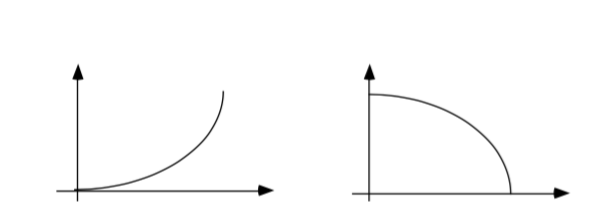
\includegraphics[scale = 0.5]{chapters/chapter04/fig04/5.png}}
\caption{Monotone linguistic quantifiers}
\label{pig:owa5}
\end{figure}
\begin{figure}[h]
\vspace{.2in}
\centering{
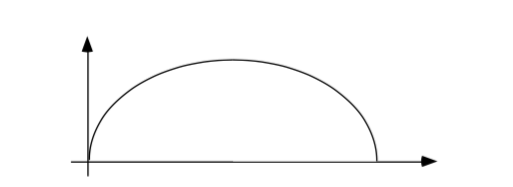
\includegraphics[scale = 0.5]{chapters/chapter04/fig04/6.png}}
\caption{Unimodal linguistic quantifier}
\label{pig:owa6}
\end{figure}

With $a_i = A_i(x)$ the overall valuation of $x$ is $F_Q(a_1,\dots,a_d)$ where $F_Q$ is an OWA operator. The weights associated with this quantified guided aggregation are obtained as follows 
\begin{equation}
\label{equa:owa5}
w_i = Q(\frac{i}{d}) - Q(\frac{i-1}{d}) , i = 1,\dots,n.
\end{equation}

From the Figure~\ref{pig:owa7} graphically shows that the operation involved in determining the OWA weights directly from the quantifier guiding the aggregation.
\begin{figure}[h]
\vspace{.2in}
\centering{
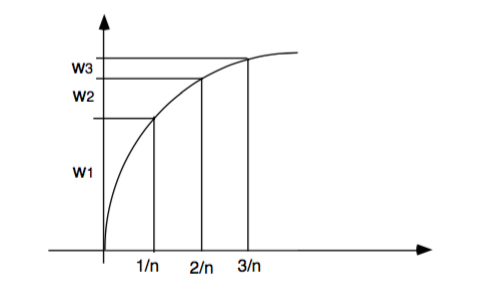
\includegraphics[scale = 0.5]{chapters/chapter04/fig04/7.png}}
\caption{Determining weights from a quantifier.}
\label{pig:owa7}
\end{figure}

Let us look at the weights generated from some basic types of quantifiers. The quantifier, for all $Q_{\ast}$ referred to the figure~\ref{pig:owa8}, is defined such that
\[Q_{\ast}(r) = \left\{
\begin{matrix}
0 & \text{for } r<1,\\
1 & \text{for } r=1.
\end{matrix}\right.\]

Using this method for generating weights
\[w_i = Q_{\ast}(\frac{i}{d})-Q_{\ast}(\frac{i-1}{d})\]
we get 
\[w_i = \left\{
\begin{matrix}
0 & \text{  for  } i<n, \\
1 & \text{  for  } i=n.
\end{matrix}
\right.\]
\begin{figure}[h]
\vspace{.2in}
\centering{
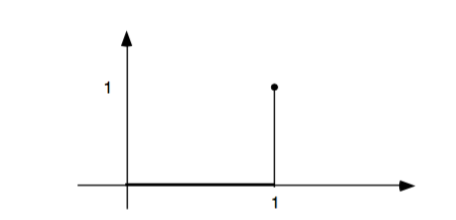
\includegraphics[scale = 0.5]{chapters/chapter04/fig04/8.png}}
\caption{The quantifier all.}
\label{pig:owa8}
\end{figure}

This is exactly what we previously denoted as $W_{\ast}$.

For the quantifier there exists (referred to the figure~\ref{pig:owa9})we have 
\[Q^{\ast}(r) = \left\{
\begin{matrix}
0 & \text{for } r=0,\\
1 & \text{for } r>0.
\end{matrix}\right.\]
\begin{figure}[h]
\vspace{.2in}
\centering{
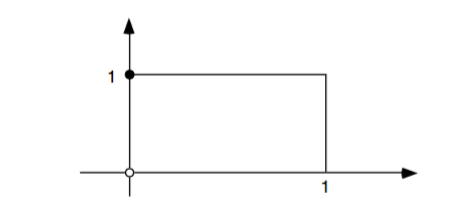
\includegraphics[scale = 0.5]{chapters/chapter04/fig04/9.png}}
\caption{The quantifier there exists.}
\label{pig:owa9}
\end{figure}

In this case we get 
\[w_1 = 1, w_i = 0, \text{  for } i\neq 1.\]
This is exactly what we denoted as $W^{\ast}$.

Consider next the quantifier referred to the figure~\ref{pig:owa10} defined by 
\[Q(r) = r.\]
\begin{figure}[h]
\vspace{.2in}
\centering{
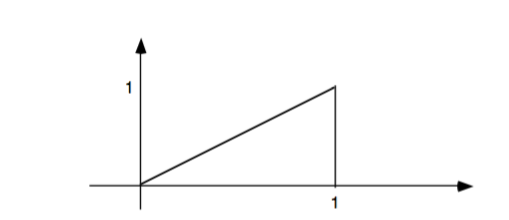
\includegraphics[scale = 0.5]{chapters/chapter04/fig04/10.png}}
\caption{The identity quantifier.}
\label{pig:owa10}
\end{figure}
This is an identity or linear type quantifier.

In this case, we get
\[w_i = Q(\frac{i}{d})-Q(\frac{i-1}{d}) = \frac{i}{d} - \frac{i-1}{d} = \frac{1}{d}.\]
This gives us the pure averaging OWA aggregation operator.

The standard degree of orness associated with a Regular Increasing Monotone (RIM) linguistic quantifier $Q$
\[\text{orness}(Q) = \int_0^1Q(r)\mathrm{d}r\]
is equal to the area under the quantifier\cite{yager1996quantifier}. This definition for the measure of orness of quantifier provides a simple useful method for obtaining this measure. 